\documentclass[12pt]{article}

\title{}

\usepackage{mymacros}

\newcommand{\bx}{\mathbf{x}}
\newcommand{\bv}{\mathbf{v}}
\newcommand{\bw}{\mathbf{w}}
\newcommand{\bA}{\mathbf{A}}
\newcommand{\bI}{\mathbf{I}}
\newcommand{\NI}{\noindent}

\begin{document}


\subsection*{Solving a linear system with repeated defective eigenvalues}

\textit{Here we do not consider the case of non-defective repeated eigenvalues, as they can be treated with the techniques of Sec. 5.2, i.e. without the use of generalized eigenvectors.}

\medskip

\noindent Below we assume that we are working with a linear system of the form
\begin{equation}
	\bx'(t)=\bA \bx(t),\label{ode}
\end{equation}
where $\bA$ is a constant $n\times n$ matrix.


\NI \textbf{The Idea:} If an eigenvalue of multiplicity $m$ has defect $\geq 1$, we won't be able to find $m$ linearly independent eigenvectors and we'll need to ``fill up the multiplicity'' with chains of generalized eigenvectors; that is, we need to find chains of generalized eigenvectors associated to $\l$ and based on linearly independent true eigenvectors such that the sum of their lengths equals the multiplicity.

\begin{example}
	Suppose we have a $4\times 4$ matrix with an eigenvalue of defect 2. 
	This means that we cannot find more than two eigenvectors which are linearly independent (the vector space formed by the eigenvectors is two dimensional).
	Schematically, we can have one of the possibilities in Fig. \ref{figure} for the chains.
	Here $v_1$, $w_1$ are true eigenvectors (generalized eigenvectors of rank 1).
	On the left, $\{v_1,v_2,v_3\}$ are a chain of length 3 based on $v_1$.
	On the right, $\{v_1, v_2\}$ and $\{w_1, w_2\}$ are chains or length two based on $v_1$, $w_1$ respectively.
	\begin{figure}[h]
	\begin{center}
		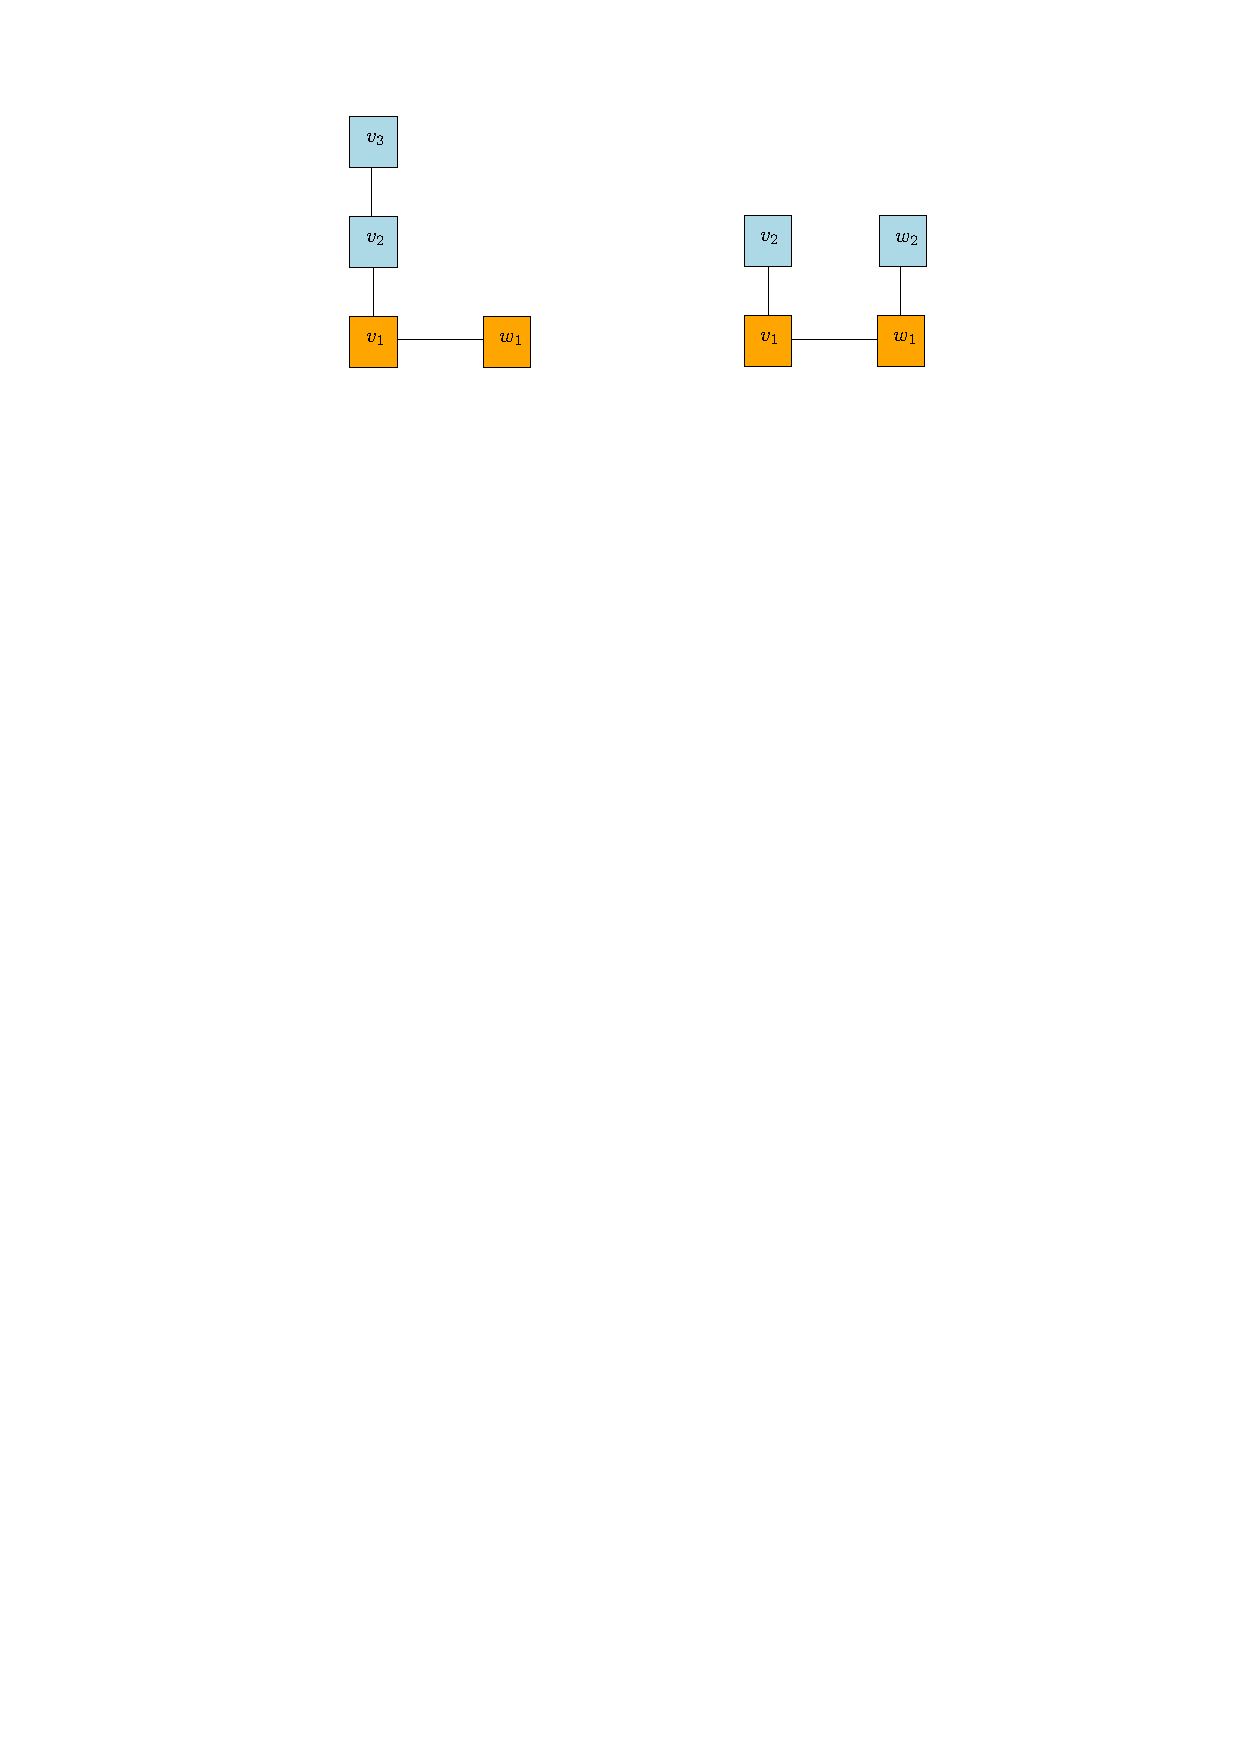
\includegraphics[scale=1]{eigenvectors.pdf}
		\end{center}
		\label{figure}
		\caption{Configurations}
	\end{figure}
	
		
\end{example}




\NI We can compute the general solution to \eqref{ode} by following the steps below:
\begin{enumerate}
	\item Compute the eigenvalues and (honest) eigenvectors associated to them. This step is needed so that you can determine the defect of any repeated eigenvalue.
	\item \label{step2} If you determine that one of the eigenvalues (call it $\l$) has multiplicity $m$ with defect $k$, try to find a chain of generalized eigenvectors of length $k+1$ associated to $\l$.

	To do so: start \emph{from the top}, i.e. try to find a generalized eigenvector of rank $k+1$ and use it to go down the chain, finding generalized eigenvectors of lower rank, until you reach an eigenvector of rank 1 (that is, an honest eigenvector).

	To find a generalized eigenvector of degree $k+1$, seek a solution $\bv_{k+1}$ satisfying the following:
	\begin{equation}\label{eq:gen_eigen}
		\begin{cases}
			(\bA-\l \bI)^{k+1}\bv_{k+1}=\mathbf{0}\\
			(\bA-\l \bI)^{k}\bv_{k+1}\neq \mathbf{0}
		\end{cases}
	\end{equation}
	If such a $\bv_{k+1}$ exists, it means you can construct a chain of generalized eigenvectors $\{v_1,\dots,v_{k+1}\}$ of length $k+1$, starting at the top and going down:
	\begin{equation}
		\label{eq:chain}
	% 
	\begin{aligned}
		&(\bA-\l \bI)\bv_{k+1}=\bv_k\\
		&(\bA-\l \bI)\bv_{k}=\bv_{k-1}\\
		&\dots\\
		&(\bA-\l \bI)\bv_{2}=\bv_{1}
	\end{aligned}
\end{equation}
Here $\bv_1$ is an honest eigenvector.

	
	\item Given a chain of leingth $k+1$, we can find $k+1$ linearly independent solutions for \eqref{ode}:
	\begin{align}
		&\bx_1(t)=e^{\l t}\bv_1\qquad \qquad \;\text{[Uses true eigenvector]}\\
		&\bx_2(t)=e^{\l t}(\bv_1 t+\bv_2)\quad \text{[True eigenvector is moved in front of the $t$]}\\
		&\dots\\
		&\bx_{k+1}(t)=e^{\l t}\big(\bv_1 \frac{t^k}{k!}+\bv_2\frac{t^{k-1}}{(k-1)!}+\dots \bv_{k}t+\bv_{k+1}\big)
	\end{align}
		
		

	\item If the multiplicity $m$ of $\l$ is larger than $k+1$, that is, if the chain we produced in step \ref{step2} does not produce $m$ generalized eigenvectors, we need to use chains of generalized eigenvectors based on true eigenvectors which are linearly independent from $\bv_1$.


	\item It might not be possible to find a length $k+1$ chain in step 2, that is, a vector $\bv_k$ in \eqref{eq:gen_eigen} might not exist (see Example \ref{example}). 
	In that case, try to find a chain of length $k$ etc. 



\end{enumerate}

\NI \textbf{Tip:} When trying to find a chain of generalized eigenvectors, always start \emph{from the top}, i.e. from the eigenvector of highest rank, and go down the chain, instead of trying to start from a true eigenvector and work your way up.



\begin{example}
	Consider $\bx'=\bA\bx$, where 
	\begin{equation}
		\bA=\left(
\begin{array}{cccc}
 3 & 1 & 0 & 0 \\
 0 & 3 & 1 & 0 \\
 0 & 0 & 3 & 0 \\
 0 & 0 & 0 & 3 \\
\end{array}
\right).
	\end{equation}
$\bA$ has eigenvalue $3$ with multiplicity 4.
Solving the system 
\begin{equation}
	(\bA-3\bI)\bv=\mathbf{0}
\end{equation} 
we find that any eigenvector $\bv=(v_1,v_2,v_3,v_4)^T$ satisfies $v_2=v_3=0$ and therefore we can find two linearly independent eigenvectors by choosing $v_1$, $v_2$ as we please.
Here we can choose, for example
\begin{equation}
	\td{\bv}_1=\begin{pmatrix}
		3\\
		0\\
		0\\
		9
	\end{pmatrix},\qquad \td{\bw}_1=\begin{pmatrix}
		1\\
		0\\
		0\\
		7
	\end{pmatrix}.
\end{equation}
We have defect 2. We try to find a length $2+1=3$ chain of generalized eigenvectors.
\emph{We start at the top}.
Try to solve
\begin{equation}\label{eq:e-vectors}
		\begin{cases}
			(\bA-3 \bI)^{3}\bv_{3}=\mathbf{0}\\
			(\bA-3 \bI)^{2}\bv_{3}\neq \mathbf{0}.
		\end{cases}
	\end{equation}
We have 
\begin{equation}
	(\bA-3 \bI)^{3}= \left(
\begin{array}{cccc}
 0 & 0 & 0 & 0 \\
 0 & 0 & 0 & 0 \\
 0 & 0 & 0 & 0 \\
 0 & 0 & 0 & 0 \\
\end{array}
\right),
	\qquad (\bA-3 \bI)^{2}=\left(
\begin{array}{cccc}
 0 & 0 & 1 & 0 \\
 0 & 0 & 0 & 0 \\
 0 & 0 & 0 & 0 \\
 0 & 0 & 0 & 0 \\
\end{array}
\right)
\end{equation}
So any $\bv_3$ works, so long as its 3rd entry is non-zero.
Take e.g. 
\begin{equation}
	\bv_3=\begin{pmatrix}
		4\\
		1\\
		1\\
		0
	\end{pmatrix}
\end{equation}
Then construct the chain from it as in Step \ref{eq:chain}:
	\begin{equation}
		\bv_2=(\bA-3\bI)\bv_3=\left(
\begin{array}{c}
 1 \\
 1 \\
 0 \\
 0 \\
\end{array}
\right), \qquad \bv_1= (\bA-3\bI)\bv_2=\left(
\begin{array}{c}
 1 \\
 0 \\
 0 \\
 0 \\
\end{array}
\right)
	\end{equation}
Note that $\bv_1$ is a true eigenvector, as expected, though not one of the ones we chose in \eqref{eq:e-vectors}. That's totally fine. Since we have constructed one chain of length 3, all we need is one more (true) eigenvector which is linearly independent from $\bv_1$. 
Take $\td{\bw}_1=(1,0,0,7)^T$ from \eqref{eq:e-vectors}.
Then four linearly independent solutions to $\bx'=\bA \bx$ are 
\begin{align}
	\td{\bx}_1(t)=e^{3t}\begin{pmatrix}
		1\\
		0\\
		0\\
		7
	\end{pmatrix},\qquad \bx_1(t)=e^{3t}\left(
\begin{array}{c}
 1 \\
 0 \\
 0 \\
 0 \\
\end{array}
\right),\qquad \bx_2(t)=e^{3t}\left(\left(
\begin{array}{c}
 1 \\
 0 \\
 0 \\
 0 \\
\end{array}
\right)t+ \left(
\begin{array}{c}
 1 \\
 1 \\
 0 \\
 0 \\
\end{array}
\right)\right)\\
% 
% 
\bx_3(t)=e^{3t}\left(\left(
\begin{array}{c}
 1 \\
 0 \\
 0 \\
 0 \\
\end{array}
\right)\frac{t^2}{2}+ \left(
\begin{array}{c}
 1 \\
 1 \\
 0 \\
 0 \\
\end{array}
\right)t+\begin{pmatrix}
		4\\
		1\\
		1\\
		0
	\end{pmatrix}\right).
\end{align}

\qed
\end{example}


\NI {You are not responsible for the following example; it is just in case you would like to understand how you can work in case you can't find a chain of length $k+1$.}

\begin{example}\label{example}
		Consider $\bx'=\bA\bx$, where 
	\begin{equation}
		\bA=\left(
\begin{array}{cccc}
 3 & 1 & 0 & 0 \\
 0 & 3 & 0 & 0 \\
 0 & 0 & 3 & 1 \\
 0 & 0 & 0 & 3 \\
\end{array}
\right).
	\end{equation}
$\bA$ has eigenvalue $3$ with multiplicity 4.
The defect is 2.
A pair of linearly independent eigenvectors is (check!)
\begin{equation}
	\td{\bv}_1=\begin{pmatrix}
		3\\
		0\\
		1\\
		0
	\end{pmatrix},\qquad \td{\bw}_1=\begin{pmatrix}
		1\\
		0\\
		4\\
		0
	\end{pmatrix}.
\end{equation}
Try to find a chain of length 3, by solving \eqref{eq:e-vectors}.
You will now notice that this is not possible! we have 
\begin{equation}
	(\bA-3 \bI)^{3}= \mathbf{0},
	\qquad (\bA-3 \bI)^{2}=\mathbf{0},
\end{equation}
so we can't hope that $(\bA-3 \bI)^{2}\bv_3\neq \mathbf{0}. $
So we fall into situation in the right hand side of Fig. \ref{figure}.
Try to find two chains of length 2. We will need to solve
\begin{equation}\label{eq:e-vectors_rank_2}
		\begin{cases}
			(\bA-3 \bI)^{2}\bv_{2}=\mathbf{0}\\
			(\bA-3 \bI)\bv_{2}\neq \mathbf{0}.
		\end{cases}
	\end{equation}
	We already computed $ (\bA-3 \bI)^{2}=\mathbf{0}$, and 
	\begin{equation}
		(\bA-3 \bI)=\left(
\begin{array}{cccc}
 0 & 1 & 0 & 0 \\
 0 & 0 & 0 & 0 \\
 0 & 0 & 0 & 1 \\
 0 & 0 & 0 & 0 \\
\end{array}
\right)
	\end{equation}
A $\bv_2$ that works is $\bv_2=\begin{pmatrix}
		0\\
		2\\
		0\\
		0
	\end{pmatrix}$.
	Building a chain from it, we find $$\bv_1=(\bA-3 \bI)\bv_2=\begin{pmatrix}
			2\\
			0\\
			0\\
			0
		\end{pmatrix}.$$
This a true eigenvector.
We need one more chain of length 2 to 'fill up' the multiplicity.
Start with a generalized eigenvector of rank 2 which solves \eqref{eq:e-vectors_rank_2} and is linearly independent from $\bv_2$.
For example take  
	\begin{equation}
	\td{\bv}_2=\begin{pmatrix}
		0\\
		1\\
		0\\
		3
	\end{pmatrix}\quad \text{ and }\quad
		\td{\bv}_1=(\bA-3 \bI)\td{\bv}_2=\begin{pmatrix}
			1\\
			0\\
			3\\
			0
		\end{pmatrix},
	\end{equation}
	which is a true eigenvector, lineraly independent from $\bv_1$.
	A set of lineraly independent solutions of $\bx'=\bA\bx$ is
	% \begin{equation}
\begin{align}
	\td{\bx}_1(t)=e^{3t}\begin{pmatrix}
		1\\
			0\\
			3\\
			0
	\end{pmatrix},
	\qquad \td{\bx}_2(t)=e^{3t}\left(\left(
\begin{array}{c}
 1\\
			0\\
			3\\
			0\\
\end{array}
\right)t+ \left(
\begin{array}{c}
 0\\
		1\\
		0\\
		3\\
\end{array}
\right)\right),\\
% 
% 
% % 
% % 
% % 
\bx_1(t)=e^{3t}\left(
\begin{array}{c}
 2 \\
 0 \\
 0 \\
 0 \\
\end{array}\right),\qquad \bx_2(t)=e^{3t}\left(\left(
\begin{array}{c}
 2\\
			0\\
			0\\
			0\\
\end{array}
\right)t+ \left(
\begin{array}{c}
 0\\
		2\\
		0\\
		0\\
\end{array}
\right)\right).
% 
% % 
% \bx_2(t)=\left(\left(
% \begin{array}{c}
%  1 \\
%  1 \\
%  0 \\
%  0 \\
% \end{array}
% \right)t+\begin{pmatrix}
% 		4\\
% 		1\\
% 		1\\
% 		0
% 	\end{pmatrix}\right)\right)\\
% % 
% % 
% % 
\end{align}\qed

\end{example}



% \newpage
% \bibliographystyle{alpha}
% \bibliography{mybib.bib}
\end{document}